\section{Web Application Prototype}

The \textbf{RoadSense} web application prototype serves as the primary interface for visualizing and interacting with road condition data. It is designed to demonstrate core functionality and validate the effectiveness of the system while prioritizing simplicity and performance over scalability in this phase.

The web application is implemented using the following modern technologies:
\begin{itemize}
	\item \href{https://reactjs.org/}{React.js}: A JavaScript library for building user interfaces.
	\item \href{https://remix.run/}{Remix}: A full-stack web framework built on React for modern web apps.
	\item \href{https://www.typescriptlang.org/}{TypeScript}: A strongly typed programming language that builds on JavaScript.
	\item \href{https://react-leaflet.js.org/}{React Leaflet}: A library for integrating Leaflet maps with React.
	\item \href{https://github.com/Leaflet/Leaflet.heat}{leaflet.heat}: A plugin for adding heatmap layers to Leaflet maps.
	\item \href{https://ui.shadcn.dev/}{shadcn/ui}: A collection of customizable components for modern UIs.
\end{itemize}

The map visualization displays road condition samples retrieved from the backend and presents them color-coded based on severity. The severity levels are categorized as follows:
\begin{itemize}
	\item \textbf{Smooth (light blue)}: Road quality score between 0 and 50.
	\item \textbf{Minor (green)}: Road quality score between 51 and 100.
	\item \textbf{Moderate (yellow)}: Road quality score between 101 and 150.
	\item \textbf{Major (orange)}: Road quality score between 151 and 200.
	\item \textbf{Severe (dark red)}: Road quality score between 201 and 250.
\end{itemize}

\noindent Users can filter samples by severity to focus on specific road conditions and toggle between a heatmap view and individual data points for a more detailed analysis.

To optimize data transfer, the application uses \textbf{PostGIS} for spatial queries, fetching only the samples visible within the map's current bounding box. This approach minimizes bandwidth usage and enhances performance, ensuring the system remains responsive even with large datasets.

The backend interaction is handled through a custom API built with \textbf{Rust}, leveraging the \textbf{Actix} framework for web services and \textbf{Diesel} for database operations. Refer to \autoref{subsec:client_server_interaction} for more details on the client-server architecture. To optimize data transfer and minimize latency, the API returns road condition samples in \texttt{JSON} format based on the client map bounds. 

The following screenshots illustrate the web application prototype:

\begin{figure}[H]
	\centering
	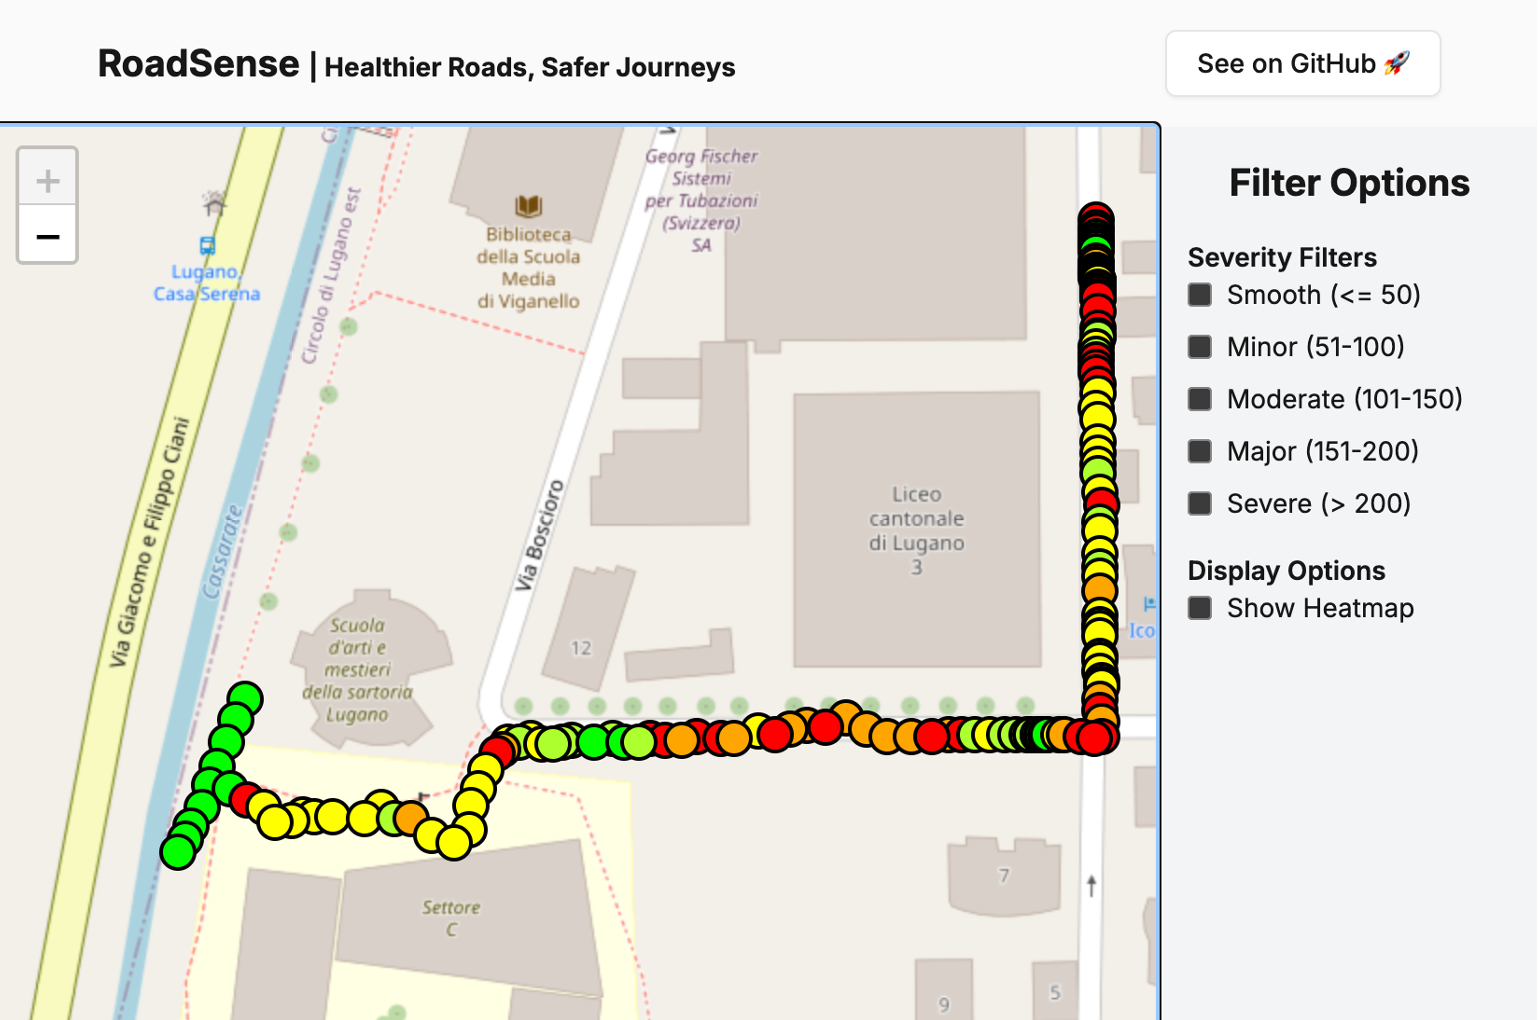
\includegraphics[width=0.9\textwidth]{../../assets/images/roadsense_webapp_points.png}
	\caption{Point Quality Data Visualization}
	\label{fig:point_quality_data}
\end{figure}

\begin{figure}[H]
	\centering
	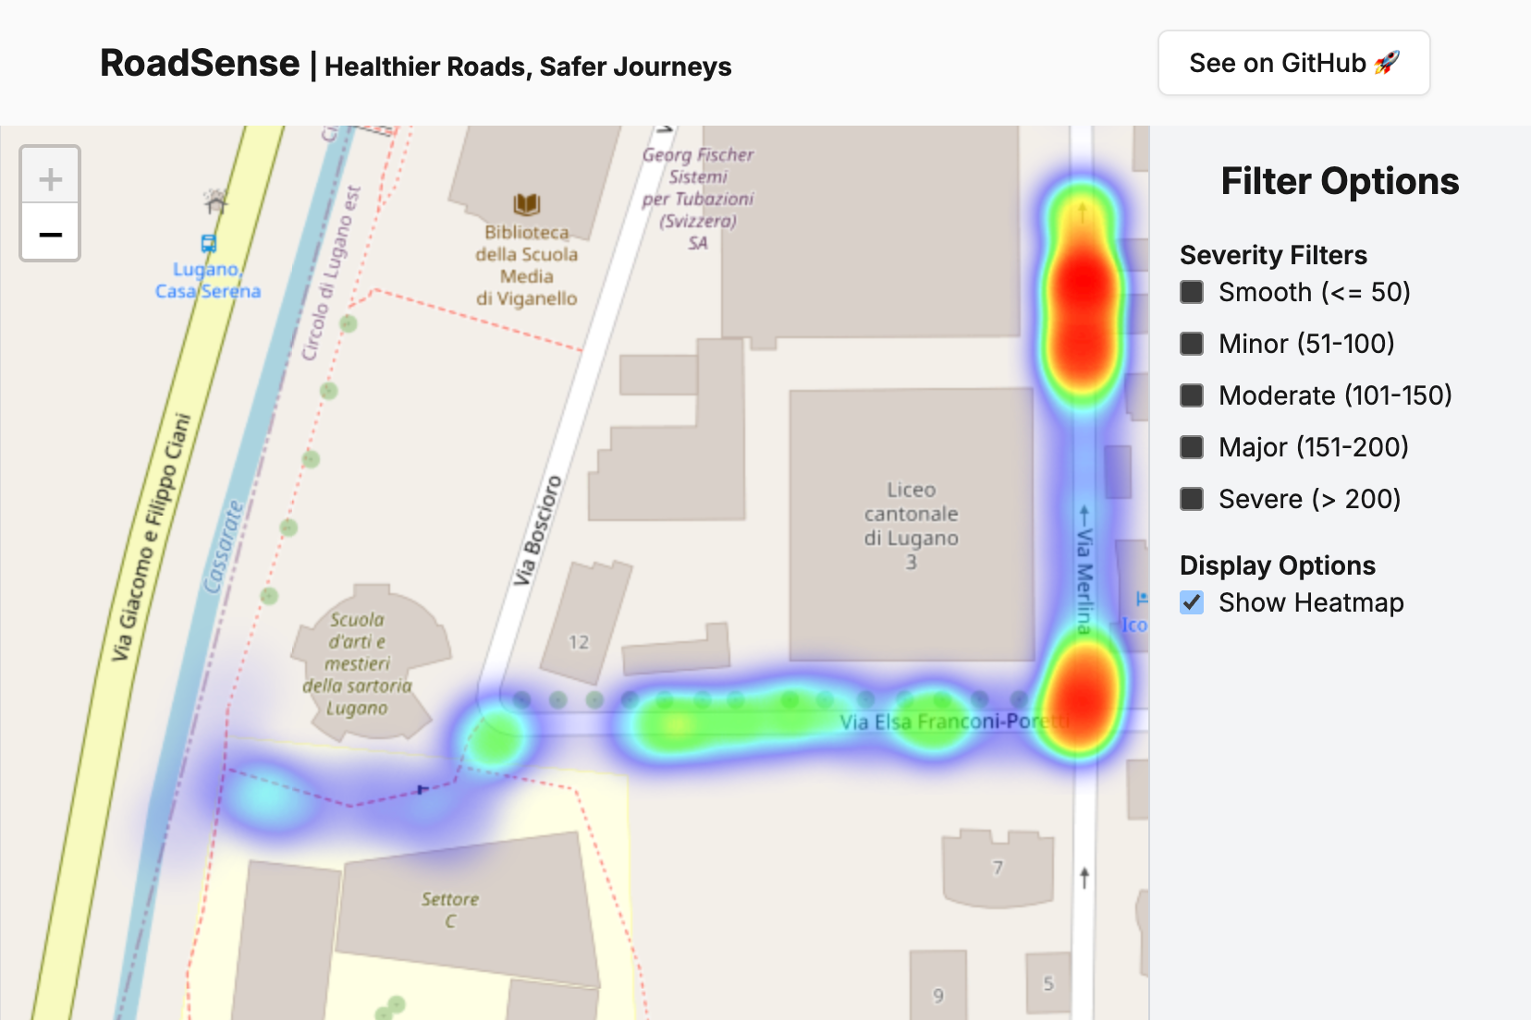
\includegraphics[width=0.9\textwidth]{../../assets/images/roadsense_webapp_heat.png}
	\caption{Data Distribution Heatmap Visualization}
	\label{fig:data_distribution_heatmap}
\end{figure}


\noindent This prototype showcases the core functionality of the \textbf{RoadSense} system, providing a foundation for future iterations that will incorporate advanced features such as user authentication, geographical-based routing, and deployment in a containerized, clustered environment.
